\documentclass[a4paper, 11pt]{article}
\usepackage[cpp]{mypackage}
\usepackage{float}
\usepackage{amsmath}
\usepackage{graphicx}
\usepackage{geometry}
\usepackage{listings}
\usepackage[colorlinks,linkcolor=red]{hyperref}
\geometry{scale=0.8}

\title{	
\normalfont \normalsize
\textsc{School of Data and Computer Science, Sun Yat-sen University} \\ [25pt] %textsc small capital letters
\rule{\textwidth}{0.5pt} \\[0.4cm] % Thin top horizontal rule
\huge  Lab2 15-Puzzle Problem (IDA*)\\ % The assignment title
\rule{\textwidth}{2pt} \\[0.5cm] % Thick bottom horizontal rule
\author{17341015 Hongzheng Chen}
\date{\normalsize\today}
}

\begin{document}
\maketitle
\tableofcontents
\newpage

\section{IDA* Algorithm}
\subsection{Description}
Iterative deepening A* (IDA*) was first described by Richard Korf in 1985, which is a graph traversal and path search algorithm that can find the shortest path between a designated start node and any member of a set of goal nodes in a weighted graph. 

It is a variant of \textbf{iterative deepening depth-first search} that borrows the idea to use a heuristic function to evaluate the remaining cost to get to the goal from the \textbf{A* search algorithm}. 

Since it is a depth-first search algorithm, its memory usage is lower than in A*, but unlike ordinary iterative deepening search, it concentrates on exploring the most promising nodes and thus does not go to the same depth everywhere in the search tree. 

\textbf{Iterative-deepening-A* works as follows:} at each iteration, perform a depth-first search, cutting off a branch when its total cost $f(n)=g(n)+h(n)$ exceeds a given threshold. This threshold starts at the estimate of the cost at the initial state, and increases for each iteration of the algorithm. At each iteration, the threshold used for the next iteration is the minimum cost of all values that exceeded the current threshold.
\subsection{Pseudocode}
\begin{figure}[ht]
\centering
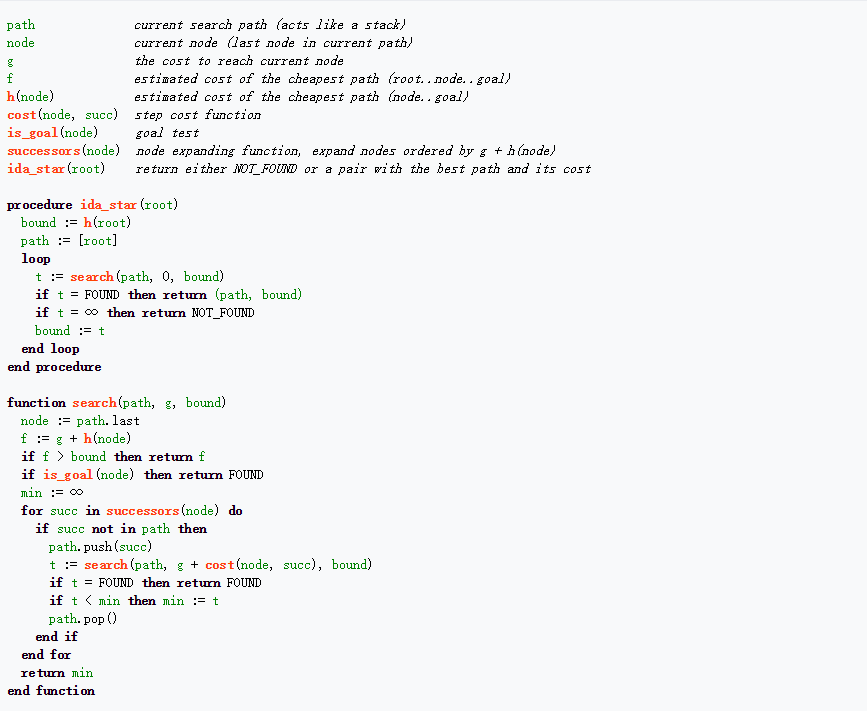
\includegraphics[width=17.3cm]{fig/code}
\end{figure}


\section{Tasks}
\begin{itemize}
	\item Please solve 15-Puzzle problem by using IDA* (Python or C++). You can use one of the two commonly used heuristic functions: h1 = the number of misplaced tiles. h2 = the sum of the distances of the tiles from their goal positions. 
	\item Here are 4 test cases for you to verify your algorithm correctness. You can also play this game (\texttt{15puzzle.zip}) for more information.
	\begin{figure}[ht]
	\centering
	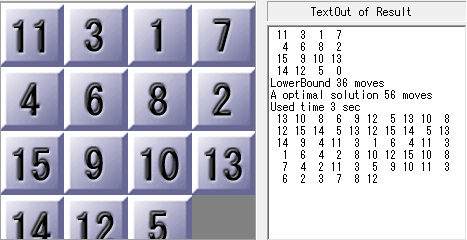
\includegraphics[width=8cm]{fig/case1}
	\quad
	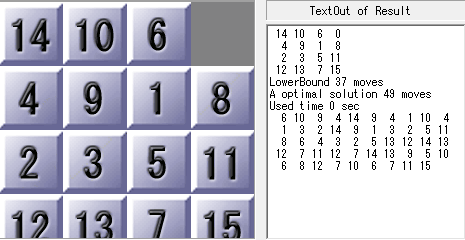
\includegraphics[width=8cm]{fig/case2}
	\\
	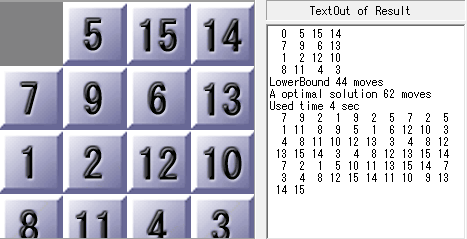
\includegraphics[width=8cm]{fig/case3}
	\quad
	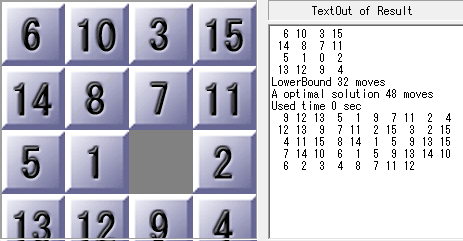
\includegraphics[width=8cm]{fig/case4}
	\end{figure}
	\item Please send \texttt{E02\_YourNumber.pdf} to \texttt{ai\_201901@foxmail.com}, you can certainly use \texttt{E02\_15puzzle.tex} as the \LaTeX template.
\end{itemize}


\section{Codes}
% In this lab, I implement the IDA$\star$ algorithm using both Python and C++.
% First is the Python code.
In this lab, I implement the IDA$\star$ algorithm in Python.
\begin{lstlisting}[language=Python]
import sys
from copy import deepcopy
from queue import PriorityQueue

MAX_INT = 0x3f3f3f3f

def print_arr(arr):
	"""
	Print arr (4*4)
	"""
	if arr == None:
		print(arr)
	else:
		for i in range(4):
			print(*(arr[i]))
	print()

def get_target_pos(num):
	"""
	Get target position of num
	"""
	return ((num-1) // 4, (num-1) % 4) if num != 0 else (3,3)

def heuristics(a):
	"""
	Heuristic function for IDA*
	"""
	res = 0
	for i in range(4):
		for j in range(4):
			(ti, tj) = get_target_pos(a[i][j])
			res += abs(i - ti) + abs(j - tj)
	return res

def find_space(a):
	"""
	Find the space of the matrix a
	"""
	for i in range(4):
		try:
			j = a[i].index(0)
			return (i,j)
		except:
			pass

def move(a,i,j,d):
	"""
	An action on matrix 'a' that moves (i,j)
	in the direction of 'd'
	"""
	res = deepcopy(a) # be careful!
	if d == 'U':
		if i+1 < 4:
			res[i][j], res[i+1][j] = res[i+1][j], res[i][j]
			return res
		else:
			return None
	elif d == 'L':
		if j+1 < 4:
			res[i][j], res[i][j+1] = res[i][j+1], res[i][j]
			return res
		else:
			return None
	elif d == 'D':
		if i-1 >= 0:
			res[i][j], res[i-1][j] = res[i-1][j], res[i][j]
			return res
		else:
			return None
	elif d == 'R':
		if j-1 >= 0:
			res[i][j], res[i][j-1] = res[i][j-1], res[i][j]
			return res
		else:
			return None
	else:
		raise RuntimeError

def search(path,cost,bound):
	"""
	Path: The previous states
	Cost: The current cost (f)
	Bound: Maximum limitation of IDA*
	"""
	arr = path[-1]
	f = cost + heuristics(arr)
	if f > bound:
		return f, False
	if arr == [[1,2,3,4],[5,6,7,8],[9,10,11,12],[13,14,15,0]]:
		return f, True # h = 0
	(si,sj) = find_space(arr)

	# find the successors
	# based on the f+g priority
	q = PriorityQueue()
	for d in ['U','L','D','R']:
		new_state = move(arr,si,sj,d) # not share
		if new_state in path:
			continue
		if new_state != None:
			priority = cost + 1 + heuristics(new_state)
			q.put((priority,new_state))

	# DFS
	minF = MAX_INT
	while not q.empty():
		_, state = q.get()
		path = path + [state]
		f, found = search(path,cost+1,bound)
		if found == True:
			return f, True
		else:
			minF = min(f,minF)
		del path[-1]
	return minF, False

def ida_star(src):
	"""
	Main function of IDA*
	"""
	bound = heuristics(arr)
	path = [src]
	while True:
		bound, found = search(path,0,bound)
		if found == True:
			break
		if bound == MAX_INT:
			print("NOT FOUND!")
			return
	print(bound)

# Read in data
arr = []
for i in range(4):
	arr.append(list(map(int,input().split())))

# Initialization
ida_star(arr)
\end{lstlisting}

% And below is the C++ Code.
% \begin{lstlisting}

% \end{lstlisting}

\section{Results}
The results are shown below.
Due to the selection of the heuristic function and the implementation language, my code cannot scale well, thus only problems within 40 steps can be solved in 1 minute.
\begin{figure}[H]
\centering
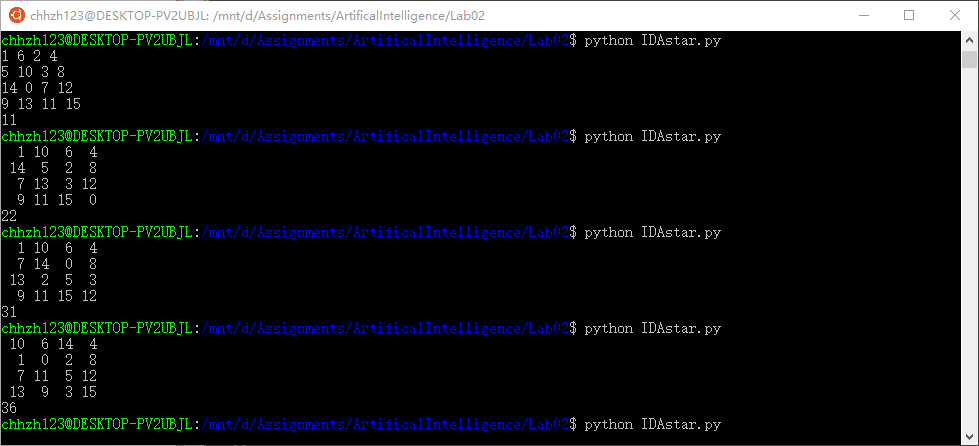
\includegraphics[width=\linewidth]{fig/python.png}
\end{figure}

% \begin{thebibliography}{99}
% \bibitem{bib1} Red Blob Games, Introduction to the A$\star$ Algorithm, \url{https://www.redblobgames.com/pathfinding/a-star/introduction.html}
% \end{thebibliography}

%\clearpage
%\bibliography{E:/Papers/LiuLab}
%\bibliographystyle{apalike}
\end{document}


% Test data

% 1 7 3 13
% 0 10 11 12
% 2 8 9 14
% 4 5 6 15

%   1  7  3 13
%   0 10 11 12
%   2  8  9 14
%   4  5  6 15
% LowerBound 37 moves
% A optimal solution 53 moves
% Used time 1 sec
%  10  7  3 13 12 11 13  3  7  8
%   9 13  8 10  2  9  5  4  9  5
%   4  6 13  4 10  7  3  8  4 14
%  11 12  8  4  7  2  5 10  6 13
%  14 11 12  8  4  3  2  6 10  9
%  13 14 15

% 1 6 2 4
% 5 10 3 8
% 14 0 7 12
% 9 13 11 15

% 1 2 3 8
% 9 7 14 13
% 5 4 6 12
% 11 0 10 15
% LowerBound 36 moves
% A optimal solution 48 moves
% Used time 0 sec
%   8  5  3 13 15 10 13 15 14 12
%   7  8  5  3 15 14 12  5  3 12
%   5  7  6  4  1  9 11 13 10  5
%   7  6  4  2  5 11  9  5  6  3
%   8  4  3  7 11 10 14 15

%   1 10  6  4
%  14  5  2  8
%   7 13  3 12
%   9 11 15  0
% 22

%   1 10  6  4
%   7 14  0  8
%  13  2  5  3
%   9 11 15 12
% 31

% 1 10 6 4
% 14 5 2 8
% 7 13 3 12
% 9 11 15 0